% ============================================================
%  ChemoInteract - Complete Project Documentation
%  Author: Ronit (Generated by Antigravity AI)
%  Version: 0.1.0
%  Compile with: pdflatex ChemoInteract_Documentation.tex
%  Run TWICE to get correct TOC and cross-references.
% ============================================================

\documentclass[12pt,a4paper,oneside]{book}

\usepackage[T1]{fontenc}
\usepackage[utf8]{inputenc}
\usepackage{lmodern}
\usepackage[margin=2.5cm]{geometry}
\usepackage{hyperref}
\usepackage{xcolor}
\usepackage{listings}
\usepackage{longtable}
\usepackage{booktabs}
\usepackage{array}
\usepackage{graphicx}
\usepackage{amsmath}
\usepackage{amssymb}
\usepackage{tikz}
\usepackage{tcolorbox}
\usepackage{fancyhdr}
\usepackage{titlesec}
\usepackage{enumitem}
\usepackage{makeidx}
\usepackage{microtype}
\usepackage{setspace}
\usepackage{caption}

\usetikzlibrary{shapes.geometric,arrows.meta,positioning,fit,backgrounds}
\tcbuselibrary{breakable,skins}
\makeindex

\hypersetup{
  colorlinks=true,
  linkcolor=blue!70!black,
  urlcolor=cyan!70!black,
  pdftitle={ChemoInteract: Complete Project Documentation},
  pdfauthor={Ronit},
  bookmarksnumbered=true,
  pdfstartview=FitH,
}

% ── Colours ──────────────────────────────────────────────────
\definecolor{codegreen}{rgb}{0,0.6,0}
\definecolor{codegray}{rgb}{0.5,0.5,0.5}
\definecolor{codepurple}{rgb}{0.58,0,0.82}
\definecolor{backcolour}{rgb}{0.97,0.97,0.97}
\definecolor{deepblue}{RGB}{0,55,120}
\definecolor{chemopurple}{RGB}{91,50,160}
\definecolor{chemogreen}{RGB}{16,140,100}
\definecolor{chemoorange}{RGB}{230,100,20}
\definecolor{noteyellow}{RGB}{255,248,200}
\definecolor{tipegreen}{RGB}{210,245,215}
\definecolor{warnorange}{RGB}{255,235,210}
\definecolor{questionblue}{RGB}{210,230,255}

% ── Listings ─────────────────────────────────────────────────
\lstdefinestyle{pythonstyle}{
  backgroundcolor=\color{backcolour},
  commentstyle=\color{codegreen}\itshape,
  keywordstyle=\color{chemopurple}\bfseries,
  numberstyle=\tiny\color{codegray},
  stringstyle=\color{chemogreen},
  basicstyle=\ttfamily\footnotesize,
  breaklines=true,
  captionpos=b,
  keepspaces=true,
  numbers=left,
  numbersep=5pt,
  showstringspaces=false,
  tabsize=4,
  frame=single,
  rulecolor=\color{gray!40},
  language=Python,
}
\lstset{style=pythonstyle}

% ── tcolorbox styles ─────────────────────────────────────────
\tcbset{
  notebox/.style={enhanced,breakable,colback=noteyellow,
    colframe=yellow!60!orange,fonttitle=\bfseries,title={Note},
    left=6pt,right=6pt,top=4pt,bottom=4pt},
  tipbox/.style={enhanced,breakable,colback=tipegreen,
    colframe=green!60!black,fonttitle=\bfseries,title={Tip},
    left=6pt,right=6pt},
  warnbox/.style={enhanced,breakable,colback=warnorange,
    colframe=orange!80!red,fonttitle=\bfseries,title={Warning},
    left=6pt,right=6pt},
  questionbox/.style={enhanced,breakable,colback=questionblue,
    colframe=blue!60!black,fonttitle=\bfseries,
    left=6pt,right=6pt,top=4pt,bottom=4pt},
  answerbox/.style={enhanced,breakable,colback=white,
    colframe=blue!30!black,
    fonttitle=\bfseries\color{blue!60!black},title={Model Answer},
    left=6pt,right=6pt},
  vivabox/.style={enhanced,breakable,colback=questionblue!40,
    colframe=deepblue,fonttitle=\bfseries,title={Viva Question},
    left=6pt,right=6pt},
  cheatbox/.style={enhanced,breakable,colback=chemopurple!8,
    colframe=chemopurple,fonttitle=\bfseries\color{white},
    coltitle=white,attach boxed title to top left,
    boxed title style={colback=chemopurple,rounded corners},
    left=6pt,right=6pt},
}

% ── Header / Footer ──────────────────────────────────────────
\pagestyle{fancy}
\fancyhf{}
\fancyhead[L]{\small\textcolor{chemopurple}{\textbf{ChemoInteract}}}
\fancyhead[R]{\small\textcolor{gray}{\leftmark}}
\fancyfoot[C]{\thepage}
\renewcommand{\headrulewidth}{0.5pt}

% ── Chapter / Section colour styles ──────────────────────────
\titleformat{\chapter}[display]
  {\normalfont\huge\bfseries\color{deepblue}}
  {\chaptertitlename\ \thechapter}{20pt}{\Huge}
\titleformat{\section}{\Large\bfseries\color{chemopurple}}{\thesection}{1em}{}
\titleformat{\subsection}{\large\bfseries\color{chemogreen}}{\thesubsection}{1em}{}
\titleformat{\subsubsection}{\normalsize\bfseries\color{chemoorange}}{\thesubsubsection}{1em}{}

\setstretch{1.2}
\setlength{\parskip}{6pt}

% ============================================================
\begin{document}

% ── Title Page ───────────────────────────────────────────────
\begin{titlepage}
\centering\vspace*{2cm}
{\Huge\bfseries\color{deepblue} ChemoInteract}\\[1cm]
{\LARGE\bfseries\color{chemopurple} Complete Project Documentation}\\[0.5cm]
{\large A Unified Deep Learning Framework for\\
Drug-Drug Interaction, Polypharmacy Side-Effect,\\
and Drug Synergy Prediction}\\[2cm]
\begin{tcolorbox}[enhanced,width=12cm,colback=deepblue!5,
  colframe=deepblue,boxrule=1.5pt,arc=8pt]
\centering
\begin{tabular}{ll}
\textbf{Author}    & Ronit \\
\textbf{Version}   & 0.1.0 \\
\textbf{Language}  & Python 3.8+ \\
\textbf{Framework} & PyTorch 2.0+ \\
\textbf{Models}    & 11 Deep Learning Architectures \\
\textbf{Datasets}  & 5 Benchmark Datasets \\
\textbf{Purpose}   & Placement / Viva / FYP Preparation \\
\end{tabular}
\end{tcolorbox}
\vfill
{\large\color{gray} Generated for Placement Interviews, College Viva,\\
Final Year Project Presentation, and Technical Discussions}
\end{titlepage}

\tableofcontents\newpage
% ================================================================
\chapter{Project Overview}\label{chap:overview}

\section{What is ChemoInteract?}

\textbf{ChemoInteract} is a deep learning library built on PyTorch. It provides a clean, modular, standardised framework for predicting what happens when two drugs are taken together. It is a research-grade software tool -- not a web application or mobile app.

When a patient takes multiple medicines at the same time, those medicines can react with each other. Some reactions are dangerous. Some make treatment more effective. ChemoInteract uses AI to \textit{predict} those reactions \textit{before} any experiment is done -- saving time, money, and potentially lives.

\begin{tcolorbox}[notebox]
ChemoInteract is a \textbf{Python library} (like NumPy or scikit-learn). You install it, import it into your Python script, and call its functions to train and evaluate models.
\end{tcolorbox}

\section{What Problem Does It Solve?}

ChemoInteract tackles three related problems in computational pharmacology:

\begin{longtable}{>{\bfseries}p{4.5cm}p{5cm}p{5cm}}
\toprule
\textbf{Problem} & \textbf{What It Means} & \textbf{Why It Matters} \\
\midrule\endhead
Drug-Drug Interaction (DDI) &
Predicting whether two drugs will interact when taken together &
Many patients take 5+ medicines daily. A bad interaction can cause serious harm or death. \\
\midrule
Polypharmacy Side Effects &
Predicting which side effects arise \textit{specifically} from combining two drugs &
These are hard to find in trials because they require specific combinations. \\
\midrule
Drug Synergy &
Predicting whether two drugs work \textit{better together} than alone &
Critical for cancer treatment --- oncologists combine drugs to kill tumour cells more effectively. \\
\bottomrule
\end{longtable}

\section{Why Was It Built?}

Before ChemoInteract, a researcher comparing five models on the same dataset had to write separate code for each model, separate data loading pipelines, training loops, and evaluation scripts. ChemoInteract solves this with a \textbf{single unified pipeline}: one call to \texttt{pipeline()} handles everything.

\section{What Makes It Unique?}

\begin{itemize}
  \item \textbf{11 models in one place} -- from simple FC networks to GNNs with attention.
  \item \textbf{5 benchmark datasets} -- all automatically downloaded and pre-processed.
  \item \textbf{One-line training} -- \texttt{pipeline()} replaces hundreds of lines of boilerplate.
  \item \textbf{Modular design} -- every component (model, dataset, optimizer, loss) can be swapped.
  \item \textbf{GPU/CPU transparency} -- automatically uses GPU if available.
  \item \textbf{Research-grade} -- each model links to its original published paper.
\end{itemize}

% ================================================================
\chapter{Folder Structure}\label{chap:folders}

\section{Root Level}

\begin{lstlisting}[language=bash]
ChemoInteract/
|-- .git/                <- Git version control metadata
|-- README.md            <- Project introduction and usage guide
|-- ChemoInteract_Main/  <- All project source code lives here
\end{lstlisting}

\section{ChemoInteract\_Main/}

\begin{lstlisting}[language=bash]
ChemoInteract_Main/
|-- ChemoInteract/   <- The actual Python library (the package)
|-- data_cleaning/   <- Scripts to download and clean raw datasets
|-- dataset/         <- Pre-processed dataset files on disk
|-- examples/        <- Example scripts showing how to use the library
|-- tests/           <- Unit tests to verify everything works
\end{lstlisting}

\subsection{ChemoInteract/ -- The Python Package}

\begin{lstlisting}[language=bash]
ChemoInteract/
|-- __init__.py        <- Package entry point; imports everything
|-- version.py         <- Stores the version: "0.1.0"
|-- constants.py       <- Shared constants (default node feature count)
|-- compat.py          <- Compatibility fixes for external libraries
|-- utils.py           <- Shared utilities (device detection, softmax)
|-- loss.py            <- Custom loss functions (CASTER)
|-- pipeline.py        <- The main pipeline() function and Result
|-- data/              <- Sub-package: data loading + batch generation
|-- models/            <- Sub-package: all 11 deep learning models
\end{lstlisting}

\subsection{data/ -- Data Sub-Package}

\begin{lstlisting}[language=bash]
data/
|-- __init__.py          <- Exports everything; creates dataset_resolver
|-- datasetloader.py     <- Abstract DatasetLoader + 5 dataset classes
|-- batchgenerator.py    <- BatchGenerator: yields DrugPairBatch objects
|-- drugfeatureset.py    <- DrugFeatureSet: drug features + molecules
|-- contextfeatureset.py <- ContextFeatureSet: cell-line gene profiles
|-- drugpairbatch.py     <- DrugPairBatch: one batch for training
|-- labeledtriples.py    <- LabeledTriples: (drug1, drug2, ctx, label)
|-- utils.py             <- Helpers: TDC download, fingerprints, JSON
\end{lstlisting}

\subsection{models/ -- Models Sub-Package}

\begin{lstlisting}[language=bash]
models/
|-- __init__.py     <- Exports all models; creates model_resolver
|-- base.py         <- Abstract Model base class
|-- deepsynergy.py  <- DeepSynergy (FC, drug features + context)
|-- deepddi.py      <- DeepDDI (FC, drug features only)
|-- matchmaker.py   <- MatchMaker (FC with shared sub-networks)
|-- deepdds.py      <- DeepDDS (GCN + MLP + context)
|-- deepdrug.py     <- DeepDrug (GCN + max readout)
|-- caster.py       <- CASTER (encoder-decoder + custom loss)
|-- gcnbmp.py       <- GCNBMP (GCN + highway + circular correlation)
|-- epgcnds.py      <- EPGCN-DS (two GCN layers + mean readout)
|-- mrgnn.py        <- MR-GNN (GCN + LSTM multi-resolution)
|-- mhcaddi.py      <- MHCADDI (multi-head co-attention)
|-- ssiddi.py       <- SSI-DDI (GCN + LSTM substructure interaction)
\end{lstlisting}

\subsection{dataset/ -- Pre-Processed Data Files}

\begin{lstlisting}[language=bash]
dataset/
|-- drugbankddi/
|   |-- drug_set.json        <- {drug_id: {smiles, features[256]}}
|   |-- context_set.json     <- {context_id: [one_hot_vector]}
|   |-- labeled_triples.csv  <- drug_1, drug_2, context, label
|-- drugcomb/    <- Same three files
|-- drugcombdb/  <- Same three files
|-- twosides/    <- Same three files
\end{lstlisting}

\begin{tcolorbox}[tipbox]
Every dataset is stored in \textbf{exactly three files}. This is the key to ChemoInteract's modularity: models just receive tensors; they do not care which dataset is used.
\end{tcolorbox}
% ================================================================
\chapter{File-by-File Explanation}\label{chap:files}

\section{version.py}
\begin{lstlisting}[language=Python]
__version__ = "0.1.0"
\end{lstlisting}
Stores the version string. Used by \texttt{pipeline.py} to record which version produced which results (reproducibility). If removed: import errors throughout the package.

\section{constants.py}
\begin{lstlisting}[language=Python]
from torchdrug.data import Molecule
from torchdrug.data.feature import atom_default
TORCHDRUG_NODE_FEATURES = len(atom_default(
    Molecule.dummy_mol.GetAtomWithIdx(0)))
\end{lstlisting}
Dynamically computes the number of atom features TorchDrug generates (typically 69). All GNN models use this constant so they remain compatible if TorchDrug changes its featurisation scheme.

\section{compat.py}
A compatibility shim layer. Three key patches:
\begin{enumerate}
  \item Patches missing \texttt{mplCanvas} attribute in older versions of RDKit.
  \item Adds \texttt{.to(device)} method to \texttt{PackedGraph} (TorchDrug's graph type lacks this, breaking GPU transfer).
  \item Adds \texttt{data\_dict} property that unifies \texttt{node\_feature} and \texttt{atom\_feature} naming differences across TorchDrug versions.
\end{enumerate}
\begin{tcolorbox}[warnbox]
If \texttt{compat.py} is removed: GNN models cannot run on GPU, and some TorchDrug versions throw \texttt{KeyError: 'node\_feature'}.
\end{tcolorbox}

\section{utils.py (root package)}
\begin{longtable}{>{\bfseries}p{4.5cm}p{10cm}}
\toprule
Function & Description \\
\midrule\endhead
\texttt{resolve\_device()} & Returns correct \texttt{torch.device}. Logs a warning and falls back to CPU if CUDA requested but unavailable. \\
\midrule
\texttt{segment\_max()} & Maximum value per graph segment. Used for numerically stable softmax in MHCADDI. \\
\midrule
\texttt{segment\_sum()} & Sum per graph segment. Used for attention normalisation in MHCADDI. \\
\midrule
\texttt{segment\_softmax()} & Softmax within each graph's node set. Subtracts segment maximum before \texttt{exp()} for overflow prevention. \\
\bottomrule
\end{longtable}

\section{pipeline.py}
The most important file in the project. Contains two key components:

\subsection{Result Dataclass}
\begin{lstlisting}[language=Python]
@dataclass
class Result:
    model: Model               # The trained PyTorch model
    predictions: pd.DataFrame  # drug_1, drug_2, context, label, prediction
    losses: List[float]        # Per-batch training losses
    train_time: float          # Seconds spent training
    evaluation_time: float     # Seconds spent evaluating
    metrics: Mapping[str, float]  # e.g. {"roc_auc": 0.872}
\end{lstlisting}
Also provides: \texttt{summarize()} (prints metrics table to console) and \texttt{save(dir)} (saves model.pkl + results.json to disk).

\subsection{pipeline() -- Step-by-Step Responsibilities}
\begin{enumerate}
  \item Resolves the device (GPU or CPU) via \texttt{resolve\_device()}
  \item Creates the dataset loader from name, class, or instance
  \item Splits data 80/20 into train and test \texttt{LabeledTriples}
  \item Creates two \texttt{BatchGenerator} objects (train + test)
  \item Instantiates (or uses provided) Model and moves it to device
  \item Creates Adam optimizer and \texttt{BCELoss} (or custom CASTER loss)
  \item Runs training loop with tqdm progress bar
  \item Evaluates on test set with \texttt{model.eval()}
  \item Computes ROC-AUC, MSE, MAE via scikit-learn
  \item Returns populated \texttt{Result} object
\end{enumerate}

\section{loss.py --- CASTERSupervisedLoss}
\[
\mathcal{L} = \mathcal{L}_{\mathrm{BCE}}(\hat{y},y)
+ \lambda_r\,\mathcal{L}_{\mathrm{BCE}}(\hat{x},x)
+ \lambda_p\!\left[\|z - C D\|_F + \lambda_1\tfrac{\|C\|_1}{N} + \lambda_2\tfrac{\|D\|_F}{N}\right]
\]
\begin{itemize}
  \item $\mathcal{L}_{\mathrm{BCE}}(\hat{y},y)$: Supervised prediction loss on interaction labels.
  \item $\mathcal{L}_{\mathrm{BCE}}(\hat{x},x)$: Reconstruction loss (autoencoder branch).
  \item Projection term: penalises poor sparse coding fit, enforces dictionary sparsity ($\ell_1$) and orthogonality ($\|D\|_F$).
\end{itemize}

\section{data/labeledtriples.py}
Wraps a Pandas DataFrame where each row is \texttt{(drug\_1, drug\_2, context, label)}.\\
Key methods:
\begin{itemize}
  \item \texttt{train\_test\_split(split=0.8, random\_state=42)}: returns two \texttt{LabeledTriples}
  \item \texttt{get\_drug\_count()}: count of unique drugs
  \item \texttt{get\_positive\_rate()}: fraction of label=1 rows
  \item \texttt{\_\_add\_\_()}: merge two \texttt{LabeledTriples} by concatenating DataFrames
\end{itemize}

\section{data/batchgenerator.py}
Python Iterator (\texttt{\_\_iter\_\_} / \texttt{\_\_next\_\_}). At each \texttt{next()} call it:
\begin{enumerate}
  \item Slices the next N rows from \texttt{LabeledTriples}
  \item Retrieves drug fingerprints, molecular graphs, context from the feature sets
  \item Packages everything into a \texttt{DrugPairBatch}
\end{enumerate}
Shuffles all rows at the start of every epoch for training randomness.

\section{data/datasetloader.py --- Class Hierarchy}
\begin{center}
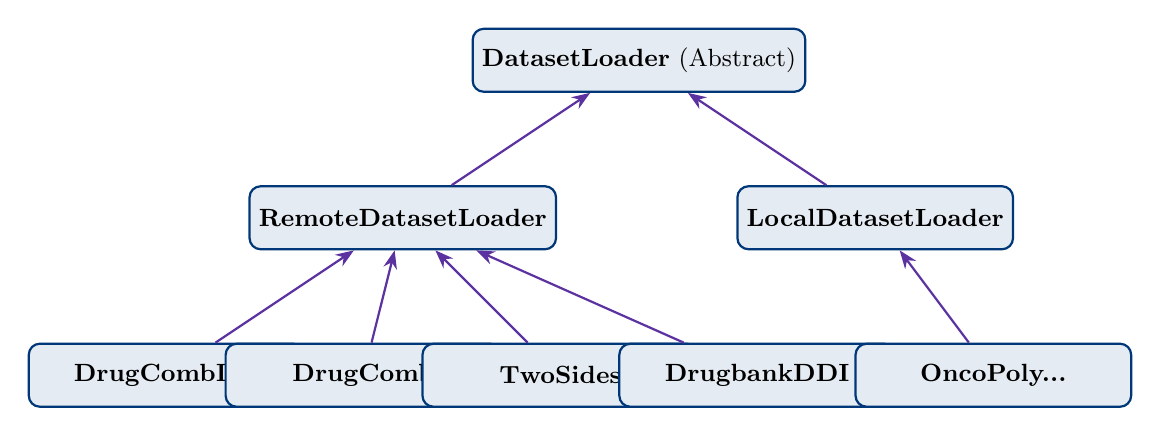
\begin{tikzpicture}[
  class/.style={rectangle,draw=deepblue,thick,fill=deepblue!10,
    rounded corners,minimum width=3.5cm,minimum height=0.8cm,
    align=center,font=\small},
  arrow/.style={-Stealth,thick,color=chemopurple},
]
  \node[class] (base) at (0,0)  {\textbf{DatasetLoader} (Abstract)};
  \node[class] (rem)  at (-3,-2) {\textbf{RemoteDatasetLoader}};
  \node[class] (loc)  at (3,-2)  {\textbf{LocalDatasetLoader}};
  \node[class] (db)   at (-6,-4) {\textbf{DrugCombDB}};
  \node[class] (dc)   at (-3.5,-4) {\textbf{DrugComb}};
  \node[class] (ts)   at (-1,-4)  {\textbf{TwoSides}};
  \node[class] (ddi)  at (1.5,-4) {\textbf{DrugbankDDI}};
  \node[class] (onco) at (4.5,-4) {\textbf{OncoPoly...}};
  \draw[arrow] (rem)  -- (base);
  \draw[arrow] (loc)  -- (base);
  \draw[arrow] (db)   -- (rem);
  \draw[arrow] (dc)   -- (rem);
  \draw[arrow] (ts)   -- (rem);
  \draw[arrow] (ddi)  -- (rem);
  \draw[arrow] (onco) -- (loc);
\end{tikzpicture}
\end{center}
Every concrete dataset class implements three abstract methods:
\texttt{get\_drug\_features()}, \texttt{get\_context\_features()}, \texttt{get\_labeled\_triples()}.\\
All three are decorated with \texttt{@lru\_cache(maxsize=1)} to prevent repeated downloads.

% ================================================================
\chapter{Technology Stack}\label{chap:techstack}

\begin{longtable}{>{\bfseries}p{3cm}p{2.5cm}p{9cm}}
\toprule
\textbf{Technology} & \textbf{Version} & \textbf{Role in ChemoInteract} \\
\midrule\endhead
Python       & 3.8+   & Entire codebase \\
PyTorch      & 2.0+   & Neural networks, tensors, autograd, GPU management \\
TorchDrug    & Latest & Molecular graph types (\texttt{PackedGraph}), GCN layers, graph readouts \\
RDKit        & Latest & SMILES string parsing, Morgan fingerprint computation \\
scikit-learn & 1.0+   & Train/test split, ROC-AUC, MSE, MAE metric computation \\
Pandas       & 1.3+   & DataFrame for labeled triples and predictions \\
NumPy        & 1.21+  & Numerical array operations throughout \\
class-resolver & Latest & String-to-class resolution for models and datasets \\
pystow       & Latest & Standardised cross-platform data directory management \\
tqdm         & 4.0+   & Training progress bars (\texttt{trange}) \\
tabulate     & 0.8+   & Console table formatting in \texttt{Result.summarize()} \\
torch-scatter & 2.0+  & Efficient scatter-add operations in GCNBMP attention pooling \\
more-itertools & 8.0+ & \texttt{chunked}, \texttt{pairwise} utilities in GCNBMP \\
click        & 7.0+   & CLI argument parsing for data cleaning scripts \\
PyTDC        & Latest & Downloading Therapeutics Data Commons benchmark datasets \\
\bottomrule
\end{longtable}

\begin{tcolorbox}[notebox]
\textbf{What is Autograd?} When you call \texttt{loss.backward()}, PyTorch automatically traces the computation graph backwards and computes gradients for every learnable parameter. You never manually derive or implement gradient equations.
\end{tcolorbox}

\begin{tcolorbox}[notebox]
\textbf{What is a Morgan Fingerprint?} A fixed-length binary vector (256 bits here) encoding which chemical substructures are present in a molecule. Computed by a circular hashing algorithm that looks up to radius 2 bonds from each atom. Similar molecules tend to have similar fingerprints.
\end{tcolorbox}

\begin{tcolorbox}[notebox]
\textbf{What is class-resolver?} It maps Python class names to the actual class objects at runtime. Writing \texttt{pipeline(model="deepsynergy")} automatically finds and instantiates \texttt{DeepSynergy}. This enables configuration-file-driven experiments and the string API.
\end{tcolorbox}
% ================================================================
\chapter{Project Workflow}\label{chap:workflow}

\section{Complete Data Flow}

\begin{center}
\begin{tikzpicture}[
  node distance=0.75cm,
  box/.style={rectangle,draw=deepblue,thick,fill=deepblue!8,rounded corners=5pt,
    minimum width=11cm,minimum height=0.75cm,align=center,font=\small},
  step/.style={rectangle,draw=chemopurple!80,thick,fill=chemopurple!8,rounded corners=3pt,
    minimum width=11cm,minimum height=0.7cm,align=center,font=\footnotesize},
  arrow/.style={-Stealth,thick,color=chemogreen},
]
\node[box]  (s1)  {User calls \texttt{pipeline(dataset=..., model=..., epochs=100)}};
\node[step,below=of s1]  (s2)  {Resolve device: CUDA available? GPU. Otherwise: CPU.};
\node[step,below=of s2]  (s3)  {Create DatasetLoader (from name, class, or instance)};
\node[step,below=of s3]  (s4)  {Load: drug\_set.json + context\_set.json + labeled\_triples.csv};
\node[step,below=of s4]  (s5)  {Split LabeledTriples: 80\% train, 20\% test (seed=42)};
\node[step,below=of s5]  (s6)  {Create two BatchGenerators (train + test)};
\node[step,below=of s6]  (s7)  {Instantiate Model and call \texttt{.to(device)}};
\node[step,below=of s7]  (s8)  {Create Adam optimizer + BCELoss (or CASTERSupervisedLoss)};
\node[box,below=of s8]   (s9)  {\textbf{Training Loop:} For each epoch, for each batch\ldots};
\node[step,below=of s9]  (s10) {BatchGenerator shuffles data; slices next N drug pairs};
\node[step,below=of s10] (s11) {Retrieve: drug features, molecular graphs, context as tensors};
\node[step,below=of s11] (s12) {Move DrugPairBatch to device};
\node[step,below=of s12] (s13) {\texttt{optimizer.zero\_grad()} --- clear previous gradients};
\node[step,below=of s13] (s14) {\texttt{model.unpack(batch)} --- extract tensors this model needs};
\node[step,below=of s14] (s15) {\texttt{model.forward(...)} --- compute predictions $\in [0,1]$};
\node[step,below=of s15] (s16) {\texttt{loss(pred, labels)} --- compute scalar loss value};
\node[step,below=of s16] (s17) {\texttt{loss.backward()} --- compute gradients via autograd};
\node[step,below=of s17] (s18) {\texttt{optimizer.step()} --- update all model weights};
\node[box,below=of s18]  (s19) {\textbf{Evaluation:} Run model on test batches (no gradients)};
\node[step,below=of s19] (s20) {Compute ROC-AUC, MSE, MAE on test predictions vs labels};
\node[box,below=of s20]  (s21) {\textbf{Return Result} object: model, predictions, losses, metrics};
\foreach \a/\b in {s1/s2,s2/s3,s3/s4,s4/s5,s5/s6,s6/s7,s7/s8,s8/s9,
                   s9/s10,s10/s11,s11/s12,s12/s13,s13/s14,s14/s15,
                   s15/s16,s16/s17,s17/s18,s18/s19,s19/s20,s20/s21}
  \draw[arrow] (\a) -- (\b);
\end{tikzpicture}
\end{center}

\section{Data Preprocessing Workflow (One-Time Setup)}
\begin{enumerate}
  \item Run: \texttt{python ddi\_cleaner.py --seed 42 --ratio 1.0}
  \item PyTDC downloads the raw DrugBank dataset from the internet
  \item Script reads all drug pairs and their SMILES strings
  \item RDKit computes 256-bit Morgan fingerprints for each unique drug
  \item Negative samples generated by rejection sampling on known positives
  \item Three output files written to \texttt{dataset/drugbankddi/}
\end{enumerate}

% ================================================================
\chapter{Step-by-Step Execution Flow}\label{chap:execution}

\section{Typical Training Run}

\begin{lstlisting}[language=Python]
from chemointeract import pipeline
from chemointeract.data import DrugCombDB
from chemointeract.models import DeepSynergy

dataset = DrugCombDB()
model = DeepSynergy(
    context_channels=dataset.context_channels,
    drug_channels=dataset.drug_channels,
)
results = pipeline(
    dataset=dataset,
    model=model,
    batch_size=5120,
    epochs=100,
    context_features=True,
    drug_features=True,
    drug_molecules=False,
    metrics=["roc_auc"],
)
results.summarize()
results.save("./output/")
\end{lstlisting}

\section{Call Chain Trace}

\begin{enumerate}
  \item \textbf{\texttt{DrugCombDB()}} constructor sets \texttt{base\_url} (GitHub raw) and \texttt{dataset\_name}. No download yet.

  \item \textbf{\texttt{DeepSynergy(N, M)}} builds \texttt{nn.Sequential}:\\
  \texttt{Linear(N+2M, 4096)} $\to$ \texttt{ReLU} $\to$ \texttt{Linear(4096,2048)} $\to$ \texttt{ReLU}\\
  $\to$ \texttt{Linear(2048,1024)} $\to$ \texttt{ReLU} $\to$ \texttt{Dropout(0.5)} $\to$ \texttt{Linear(1024,1)} $\to$ \texttt{Sigmoid}

  \item \textbf{\texttt{pipeline()}} enters \texttt{pipeline.py}:
  \begin{enumerate}
    \item \texttt{resolve\_device(None)} --- tries CUDA, falls back to CPU with warning.
    \item \texttt{get\_labeled\_triples()} --- fetches CSV from GitHub via \texttt{urllib.request}; result is \texttt{@lru\_cache}'d.
    \item \texttt{train\_test\_split(0.8, random\_state=42)}.
    \item Two \texttt{BatchGenerator} objects created.
    \item \texttt{model.to(device)} moves all PyTorch parameters to GPU memory.
    \item \texttt{Adam(model.parameters(), lr=0.001)}.
    \item \texttt{BCELoss()}.
    \item \texttt{trange(100)} outer loop begins; \texttt{tqdm} shows progress bar.
  \end{enumerate}

  \item \textbf{Per-batch inner loop:}
  \begin{enumerate}
    \item \texttt{next(train\_gen)} --- slices next 5120 rows.
    \item Retrieves tensors:\\
      \texttt{drug\_features\_left} shape (5120, 256)\\
      \texttt{drug\_features\_right} shape (5120, 256)\\
      \texttt{context\_features} shape (5120, ctx\_dim)\\
      \texttt{labels} shape (5120, 1)
    \item \texttt{batch.to(device)}.
    \item \texttt{model.unpack(batch)} returns \texttt{(context, left, right)}.
    \item \texttt{model.forward(context, left, right)}:
    \begin{itemize}
      \item \texttt{torch.cat([context, left, right], dim=1)} $\to$ shape (5120, ctx+512)
      \item Pass through \texttt{nn.Sequential} layers $\to$ shape (5120, 1), values in $[0,1]$
    \end{itemize}
    \item \texttt{BCELoss(pred, labels)} $\to$ scalar loss.
    \item \texttt{loss.backward()} $\to$ \texttt{optimizer.step()}.
  \end{enumerate}

  \item \textbf{Evaluation phase:} \texttt{model.eval()} is called. Test batches are processed
  with \texttt{torch.no\_grad()}. Predictions collected, \texttt{roc\_auc\_score()} computed.

  \item \texttt{Result(...)} constructed and returned to the caller.
\end{enumerate}
% ================================================================
\chapter{Datasets}\label{chap:datasets}

\section{The Five Datasets}

\begin{longtable}{>{\bfseries}p{3.5cm}p{2.2cm}p{2.5cm}p{2cm}p{3.8cm}}
\toprule
\textbf{Dataset} & \textbf{Task} & \textbf{Loader} & \textbf{Context} & \textbf{Notes} \\
\midrule\endhead
DrugCombDB & Drug Synergy & Remote & Cell lines & Anti-cancer drug combination database \\
DrugComb & Drug Synergy & Remote & Cell lines & FIMM drug combination dataset \\
TwoSides & Side Effects & Remote & Effect types & Top-10 polypharmacy side effects \\
DrugbankDDI & DDI & Remote & Interaction types & Binary interaction labels \\
OncoPolyPharmacology & Drug Synergy & Local (TDC) & Cancer cell lines & O'Neil 2016 screen \\
\bottomrule
\end{longtable}

\section{Dataset Storage Format}

Every dataset is stored in exactly three files in its subdirectory:

\begin{lstlisting}[language=bash]
drug_set.json        <- {"drug_id": {"smiles": "...", "features": [256 floats]}}
context_set.json     <- {"context_id": [float, float, ...]}
labeled_triples.csv  <- columns: drug_1, drug_2, context, label
\end{lstlisting}

\section{Negative Sampling}

Positive samples come directly from biomedical databases. Negatives are generated by rejection sampling to avoid accidentally including known positive interactions:

\begin{lstlisting}[language=Python]
for _ in range(n_negatives):
    drug_1, drug_2 = rng.sample(all_drugs, 2)
    context = rng.choice(all_contexts)
    # Reject if this triplet is a known positive
    while (drug_1, drug_2, context) in known_positives_map:
        drug_1, drug_2 = rng.sample(all_drugs, 2)
        context = rng.choice(all_contexts)
    negative_samples.append((drug_1, drug_2, context, 0.0))
\end{lstlisting}

\begin{tcolorbox}[warnbox]
This uses the \textbf{Closed-World Assumption (CWA)}: any drug pair not found in the database is labelled 0 (non-interacting). This may introduce \textbf{false negatives}: pairs that genuinely interact but have not been experimentally tested yet.
\end{tcolorbox}

\section{Connecting a New Dataset}

To add a sixth dataset, you would:
\begin{enumerate}
  \item Write a cleaning script under \texttt{data\_cleaning/}
  \item Create \texttt{dataset/mynewdataset/} with the three standard files
  \item Create a new class inheriting \texttt{RemoteDatasetLoader} or \texttt{LocalDatasetLoader}
  \item Implement the three abstract methods
  \item Import the class in \texttt{data/\_\_init\_\_.py}
\end{enumerate}
No other file needs modification --- \texttt{pipeline.py} and all models remain untouched.

% ================================================================
\chapter{Models -- AI and Deep Learning}\label{chap:models}

\section{The Model Base Class}

\begin{lstlisting}[language=Python]
class Model(nn.Module, ABC):
    @abstractmethod
    def unpack(self, batch: DrugPairBatch):
        """Select which fields from the batch this model needs."""
        ...
    def forward(self, *args) -> torch.FloatTensor:
        """Forward pass; returns predictions in [0,1]."""
        ...
\end{lstlisting}

\texttt{unpack()} is the key design decision. The pipeline always passes the full \texttt{DrugPairBatch} object. Each model returns only the tuple it needs. This decouples \texttt{pipeline.py} from model internals entirely.

\section{Category 1: Fully Connected (FC) Models}

\subsection{DeepSynergy (Preuer et al., 2018)}
Concatenates context features + left drug fingerprint + right drug fingerprint, then feeds through four fully-connected layers:
\[
\text{Input} = [\text{ctx}\|\text{left}\|\text{right}] \in \mathbb{R}^{C+2D}
\quad\xrightarrow{4\times\mathrm{Linear+ReLU+Dropout}}\quad
\hat{y} = \sigma(W_4 \cdot h_3) \in [0,1]
\]

\subsection{DeepDDI (Ryu et al., 2018)}
Nine-layer FC network. Input: $[\text{left} \| \text{right}]$ (no context). BatchNorm applied after the first layer. Output is 86-dimensional (one per interaction type) but here used as binary predictor.

\subsection{MatchMaker (Kuru et al., 2021)}
Shared sub-network processes each drug with context \textit{independently}:
\begin{enumerate}
  \item \texttt{drug\_ctx\_layer($[\text{left} \| \text{ctx}]$)} $\to h_L$
  \item \texttt{drug\_ctx\_layer($[\text{right} \| \text{ctx}]$)} $\to h_R$ \quad (same weights as step 1!)
  \item \texttt{final\_layer($[h_L \| h_R]$)} $\to \hat{y}$
\end{enumerate}
Weight sharing enforces that each drug is processed symmetrically.

\section{Category 2: Graph Neural Network (GNN) Models}

\begin{tcolorbox}[notebox]
\textbf{GCN Layer Formula:}
\[h_v^{(l+1)} = \sigma\!\left(W^{(l)} \cdot \frac{1}{|\mathcal{N}(v)|} \sum_{u \in \mathcal{N}(v)\cup\{v\}} h_u^{(l)}\right)\]
After $k$ GCN layers, each atom's representation encodes information from its $k$-hop neighbourhood. ChemoInteract uses TorchDrug's built-in \texttt{GraphConvolution} and \texttt{GraphConvolutionWithEdge} layers.
\end{tcolorbox}

\subsection{DeepDDS (Wang et al., 2021)}
Three parallel encoders:
\begin{itemize}
  \item Cell line: $\text{ctx} \xrightarrow{\ell_2\text{-norm} + \text{MLP}} \mathbb{R}^{32}$
  \item Left drug: $\text{graph} \xrightarrow{\text{GCN} + \text{MaxReadout} + \text{MLP}} \mathbb{R}^{32}$
  \item Right drug: same GCN branch (shared weights) $\to \mathbb{R}^{32}$
\end{itemize}
All three concatenated: $[\text{ctx}_{32} \| \text{left}_{32} \| \text{right}_{32}] \xrightarrow{\text{FC}} [0,1]$

\subsection{DeepDrug (Cao et al., 2020)}
Four GCN layers per drug $\to$ Global Max Pooling $\to$ concatenate both drug representations $\to$ BatchNorm + Dropout + Linear + Sigmoid.

\subsection{CASTER (Huang et al., 2020)}
Dictionary learning / sparse coding approach:
\begin{enumerate}
  \item Input: \textit{union} of both drugs' substructure fingerprints (bit OR)
  \item FC Encoder $\to$ latent $z$
  \item Sparse coding: $c = (D^TD + \lambda I)^{-1} D^T z$ (closed-form solution)
  \item FC Decoder reconstructs $\hat{x}$ (autoencoder branch)
  \item 8-layer FC predictor $\to$ sigmoid $\to \hat{y}$
  \item Loss: prediction + reconstruction + projection (see Chapter 3)
\end{enumerate}

\subsection{GCNBMP (Chen et al., 2020)}
Three novel components:
\begin{itemize}
  \item \textbf{Highway Network:} $\mathbf{y} = T \odot H(\mathbf{x}) + (1-T) \odot \mathbf{x}$, where gate $T = \sigma(W_T \mathbf{x} + b_T)$ and $b_T = -2$ (biases toward skip-connections for stable training).
  \item \textbf{Attention Pooling:} Weighted node aggregation using \texttt{torch-scatter}.
  \item \textbf{Circular Correlation:} $(a\star b)[k] = \mathcal{F}^{-1}(\overline{\mathcal{F}(a)} \odot \mathcal{F}(b))$ via FFT for $O(n\log n)$ vs $O(n^2)$.
\end{itemize}

\subsection{EPGCN-DS (Sun et al., 2020)}
Two stacked GCN layers with Mean Readout. Combines both drug representations by \textit{element-wise addition} (Deep Sets principle): order-invariant, $\text{left} + \text{right} = \text{right} + \text{left}$.

\subsection{MR-GNN (Xu et al., 2019)}
Multi-resolution approach with two LSTMs:
\begin{itemize}
  \item \textbf{Border LSTM:} Sequences the node-level representations across GCN layers, capturing how individual drug features evolve with depth.
  \item \textbf{Middle LSTM:} Sequences the \textit{paired} drug representations, capturing how the relationship between two drugs evolves across layers.
\end{itemize}
Final prediction combines both LSTM outputs.

\section{Category 3: Attention Models}

\subsection{MHCADDI (Deac et al., 2019)}
Co-attention between two drug molecules. For each atom $i$ in drug A and atom $j$ in drug B:
\[
e_{ij}=\frac{(W_K h_i)^T(W_K h_j)}{\sqrt{d}},\quad
\alpha_{ij}=\mathrm{softmax}_{j \in B}(e_{ij}),\quad
m_i=\sum_{j \in B} \alpha_{ij}W_V h_j
\]
Atom $i$ in drug A gets a new representation $m_i$ by attending to all atoms in drug B.\\
Key difference: the two drugs are processed \textbf{jointly}, not independently.

\subsection{SSI-DDI (Nyamabo et al., 2021)}
Stacked GCN + LSTM layers specifically modelling substructure-substructure interactions. Each substructure from drug A is matched against substructures from drug B through an interaction layer.

\section{Model Capability Summary}

\begin{longtable}{>{\bfseries}p{2.8cm}p{1.8cm}p{2cm}p{2.2cm}p{2.4cm}p{2cm}}
\toprule
\textbf{Model} & \textbf{Type} & \textbf{Drug Feat.} & \textbf{Molecules} & \textbf{Context} & \textbf{Custom Loss} \\
\midrule\endhead
DeepSynergy & FC  & Yes & & Yes & \\
DeepDDI     & FC  & Yes & & & \\
MatchMaker  & FC  & Yes & & Yes & \\
DeepDDS     & GNN & & Yes & Yes & \\
DeepDrug    & GNN & & Yes & & \\
CASTER      & GNN & Yes & & & Yes \\
GCNBMP      & GNN & & Yes & & \\
EPGCN-DS    & GNN & & Yes & & \\
MR-GNN      & GNN & & Yes & & \\
MHCADDI     & Attn & & Yes & & \\
SSI-DDI     & Attn & & Yes & & \\
\bottomrule
\end{longtable}
% ================================================================
\chapter{Algorithms Deep Dive}\label{chap:algorithms}

\section{Morgan Fingerprint Algorithm}
Circular algorithm with radius $r=2$, output 256 bits:
\begin{enumerate}
  \item Assign each atom an initial integer identifier based on atomic number, charge, isotope, ring membership.
  \item For $r$ rounds: each atom combines its current identifier with the identifiers of all directly bonded atoms using a hash function.
  \item Map each resulting identifier to a bit position in a 256-bit vector via modular hashing.
  \item The final vector has 1 at position $k$ if any atom's radius-2 environment hashed to $k$.
\end{enumerate}
\textbf{Time complexity:} $O(|V| \cdot r \cdot \bar{d})$ where $\bar{d}$ is average atom degree.\\
\textbf{Space complexity:} $O(256)$ per molecule (fixed-size output).

\section{Graph Convolutional Network (GCN)}
\[h_v^{(l+1)} = \sigma\!\left(W^{(l)} \cdot \frac{1}{|\mathcal{N}(v)|} \sum_{u \in \mathcal{N}(v)\cup\{v\}} h_u^{(l)}\right)\]
\begin{itemize}
  \item $h_v^{(l)}$: feature vector of atom $v$ at layer $l$. Initially the 69-dimensional atom feature from TorchDrug.
  \item $\mathcal{N}(v)$: set of neighbouring atoms (bonded atoms).
  \item $W^{(l)}$: learnable weight matrix for layer $l$.
  \item $\sigma$: nonlinearity (usually ReLU).
  \item Self-loop (including $v$ in the sum) prevents the atom from forgetting its own features.
\end{itemize}
\textbf{Time complexity:} $O(|E| \cdot d^2)$ per layer ($|E|$ = bond count, $d$ = feature dimension).

\section{Graph Readout Functions}
After $k$ GCN layers, the model needs one vector per molecule (not one per atom):
\begin{itemize}
  \item \textbf{Max Readout:} $h_G = \max_{v \in V} h_v^{(k)}$ --- element-wise maximum over all atoms. Captures the most prominent feature. Used by DeepDrug.
  \item \textbf{Mean Readout:} $h_G = \frac{1}{|V|} \sum_{v \in V} h_v^{(k)}$ --- average. Smoother signal. Used by EPGCN-DS.
  \item \textbf{Attention Readout:} $h_G = \sum_v \alpha_v h_v^{(k)}$ --- learned weights $\alpha_v$ per atom. Used by GCNBMP.
\end{itemize}

\section{Circular Correlation (GCNBMP)}
\[(a\star b)[k] = \sum_{j=0}^{n-1} a[j] \cdot b[(j+k)\bmod n], \quad k=0,\ldots,n-1\]
\begin{itemize}
  \item Same output size as input (unlike concatenation which doubles size).
  \item Captures feature alignment at different offsets.
  \item Implemented via FFT: $a\star b = \mathcal{F}^{-1}(\overline{\mathcal{F}(a)} \odot \mathcal{F}(b))$.
  \item Complexity: $O(n\log n)$ via FFT vs $O(n^2)$ naively.
\end{itemize}

\section{Highway Network Gate (GCNBMP)}
\[\mathbf{y} = T \odot H(\mathbf{x}) + (1-T) \odot \mathbf{x}\]
where:
\begin{itemize}
  \item $H(\mathbf{x})$: the regular transformation (e.g.\ FC + ReLU).
  \item $T = \sigma(W_T \mathbf{x} + b_T)$: the learned transform gate, initialised with $b_T=-2$ to bias toward pass-through at training start.
  \item $(1-T)$: the carry gate (complement).
\end{itemize}
This provides gradient highways through deep networks, solving vanishing gradient problems.

\section{Segment Softmax (MHCADDI Attention)}
In MHCADDI, each molecular graph has a different number of atoms. Attention must be normalised \textit{per graph}, not globally. This is done with segment softmax:
\[\alpha_{ij} = \frac{\exp(e_{ij})}{\sum_{k \in \mathcal{N}(i)} \exp(e_{ik})}\]
Using the log-sum-exp trick (subtract segment maximum before \texttt{exp()}) for numerical stability. Implemented in \texttt{utils.segment\_softmax()}.

\section{Adam Optimiser}
\[m_t = \beta_1 m_{t-1} + (1-\beta_1)g_t \quad (\text{first moment estimate})\]
\[v_t = \beta_2 v_{t-1} + (1-\beta_2)g_t^2 \quad (\text{second moment estimate})\]
\[\hat{m}_t = \frac{m_t}{1-\beta_1^t}, \quad \hat{v}_t = \frac{v_t}{1-\beta_2^t} \quad (\text{bias correction})\]
\[\theta_t = \theta_{t-1} - \frac{\alpha}{\sqrt{\hat{v}_t}+\epsilon}\hat{m}_t\]
Defaults: $\alpha=0.001$, $\beta_1=0.9$, $\beta_2=0.999$, $\epsilon=10^{-8}$.

Adam adapts the learning rate per parameter. Parameters with large recent gradients get smaller effective steps. This is especially useful in GNN training where some parameters see sparse gradients.

\section{Binary Cross-Entropy (BCE) Loss}
\[\mathcal{L}_{\mathrm{BCE}} = -\frac{1}{N}\sum_{i=1}^N\left[y_i\log\hat{y}_i + (1-y_i)\log(1-\hat{y}_i)\right]\]
\begin{itemize}
  \item $y_i \in \{0,1\}$: true label.
  \item $\hat{y}_i \in (0,1)$: model probability output (after Sigmoid).
  \item Penalises confident wrong predictions most: $\log(0.01) = -4.6$ vs $\log(0.9) = -0.1$.
\end{itemize}

% ================================================================
\chapter{Security, Error Handling, and Common Issues}\label{chap:security}

\begin{tcolorbox}[notebox]
ChemoInteract is a research library, not a production service. There is no user authentication, no database server, no web API. Security considerations are therefore narrower than for a web application.
\end{tcolorbox}

\section{Security Model}

\begin{longtable}{>{\bfseries}p{4cm}p{10cm}}
\toprule
Concern & How It Is Handled \\
\midrule\endhead
Remote downloads & Data is fetched only from a hardcoded GitHub raw URL. No user-supplied URLs are accepted. \\
\midrule
Dataset name validation & \texttt{assert name in ["drugcombdb", "drugcomb", "twosides", "drugbankddi"]} fast-fails on typos. \\
\midrule
Model persistence & \texttt{torch.save()} uses Python pickle. Never load a \texttt{model.pkl} file from an untrusted source. \\
\midrule
No secrets & No API keys, \texttt{.env} files, or credentials required. \\
\bottomrule
\end{longtable}

\section{Error Handling Patterns}

\begin{lstlisting}[language=Python]
# Pattern 1: Fast-fail input validation
assert dataset_name in ["drugcombdb", "drugcomb", "twosides", "drugbankddi"]

# Pattern 2: Graceful degradation with logging
if not torch.cuda.is_available():
    logger.warning("No CUDA device found. CPU will be used.")
    device = torch.device("cpu")

# Pattern 3: Flexible output handling (CASTER returns 6-tuple)
prediction = model(...)
if isinstance(prediction, (list, tuple)):
    prediction = prediction[0]  # extract the interaction probability
\end{lstlisting}

\section{Common Runtime Errors and Solutions}

\begin{longtable}{>{\bfseries}p{3.5cm}p{5cm}p{5.5cm}}
\toprule
Error & Root Cause & Solution \\
\midrule\endhead
\texttt{AssertionError} & Misspelled dataset name & Use exact string: drugcombdb, drugcomb, twosides, drugbankddi \\
\texttt{ConnectionError} & No internet connection & Connect to internet; data is cached after first successful download \\
\texttt{CUDA out of memory} & \texttt{batch\_size} too large for GPU VRAM & Reduce \texttt{batch\_size} (try 512 or 256) \\
\texttt{size mismatch} & Wrong \texttt{context\_channels} or \texttt{drug\_channels} & Always use \texttt{dataset.context\_channels} and \texttt{dataset.drug\_channels} \\
\texttt{KeyError: node\_feature} & TorchDrug version mismatch & Ensure \texttt{compat.py} is imported at startup \\
\texttt{AttributeError: mplCanvas} & Old RDKit version & Same fix: \texttt{compat.py} patches this \\
\bottomrule
\end{longtable}
% ================================================================
\chapter{Deployment and Testing}\label{chap:deployment}

\section{Local Installation}

\begin{lstlisting}[language=bash]
git clone https://github.com/your-username/ChemoInteract.git
cd ChemoInteract/ChemoInteract_Main

# Create isolated Python environment
python -m venv venv
venv\Scripts\activate          # Windows

# Install all dependencies
pip install torch torchdrug rdkit scikit-learn pandas numpy
pip install class-resolver pystow tqdm tabulate torch-scatter
pip install more-itertools click PyTDC

# Install ChemoInteract itself in editable mode
pip install -e .

# Quick test
python examples/deepsynergy_example.py
\end{lstlisting}

\section{Running the Test Suite}

\begin{lstlisting}[language=bash]
python -m pytest tests/ -v
\end{lstlisting}

\begin{longtable}{>{\bfseries}p{5cm}p{9cm}}
\toprule
Test File & What It Covers \\
\midrule\endhead
\texttt{test\_models.py} & Forward pass of all 11 models; CASTER custom loss; model inherits from \texttt{Model}; docstrings reference original papers. \\
\texttt{test\_data\_structures.py} & \texttt{LabeledTriples} CRUD; \texttt{DrugFeatureSet} get/set; \texttt{ContextFeatureSet} shapes. \\
\texttt{test\_batching.py} & \texttt{BatchGenerator} output tensor shapes; all-False feature flags (model receives empty tensors). \\
\texttt{test\_compat.py} & \texttt{PackedGraph.to(device)} CPU-to-CPU transfer; GPU test if CUDA available. \\
\bottomrule
\end{longtable}

\section{Saving and Loading Results}

\begin{lstlisting}[language=Python]
# After training:
results = pipeline(dataset=dataset, model=model, epochs=100)

# Save both the model and metrics
results.save("./output/")
# Creates: ./output/model.pkl  (PyTorch model state)
#          ./output/results.json (metrics, train_time, losses)

# Load model for inference:
import torch
model = torch.load("./output/model.pkl")
model.eval()
\end{lstlisting}

\begin{tcolorbox}[warnbox]
\texttt{torch.load()} uses Python pickle internally. Only load \texttt{model.pkl} files from sources you trust. A maliciously crafted pickle file can execute arbitrary code.
\end{tcolorbox}

\section{GPU vs CPU Performance}

\begin{longtable}{>{\bfseries}p{3.5cm}p{5.5cm}p{5cm}}
\toprule
Model Category & CPU (batch=512, 10 epochs) & GPU (batch=5120, 100 epochs) \\
\midrule\endhead
FC models & Minutes (fast) & Seconds per epoch \\
GNN models & Tens of minutes & Minutes total \\
Attention models & Slower (graph ops) & Minutes total \\
\bottomrule
\end{longtable}

% ================================================================
\chapter{Interview Preparation}\label{chap:interview}

\section{HR / Behavioural Questions}

\begin{tcolorbox}[questionbox,title={Q1: Tell me about your final year project.}]
\end{tcolorbox}
\begin{tcolorbox}[answerbox]
``I built ChemoInteract, a deep learning library that predicts drug-drug interactions. The motivation is clinically relevant: adverse drug reactions cause thousands of preventable hospitalisations annually, particularly in elderly patients taking multiple medications simultaneously.

The core technical contribution: I unified eleven published deep learning models -- from simple fully-connected networks to graph neural networks and attention mechanisms -- in a single framework. A researcher can swap any model with a one-line change. I also integrated five real-world benchmark datasets that automatically download and pre-process.

This project demonstrates my ability to read research papers and translate them into working code, design modular software architecture, and apply deep learning to a concrete healthcare problem.''
\end{tcolorbox}

\begin{tcolorbox}[questionbox,title={Q2: What was your biggest technical challenge?}]
\end{tcolorbox}
\begin{tcolorbox}[answerbox]
``The hardest challenge was making all eleven models work within the same training pipeline despite having fundamentally different input requirements. Some models take fingerprint vectors; others take molecular graphs. Some need cell-line context; others do not. CASTER returns a 6-tuple of tensors, not a single prediction.

I solved this with two design patterns. First, the \texttt{unpack()} method: each model declares exactly what it needs from the batch by returning a tuple, so the pipeline needs zero model-specific branching. Second, \texttt{DrugPairBatch} always carries all possible data types; each model picks only what it needs. This is the Template Method design pattern.''
\end{tcolorbox}

\begin{tcolorbox}[questionbox,title={Q3: How did you validate your results?}]
\end{tcolorbox}
\begin{tcolorbox}[answerbox]
``I used ROC-AUC as the primary metric because the dataset is class-imbalanced (many more non-interacting pairs than interacting ones). Plain accuracy is misleading: a model that always predicts ``no interaction'' gets high accuracy but is useless.

I also wrote a unit test suite (\texttt{pytest}) with four test files covering all 11 model forward passes, data structure integrity, batch generation shapes, and GPU compatibility. Tests run on synthetic toy data so they do not require downloading datasets.''
\end{tcolorbox}

\section{Technical Questions}

\begin{tcolorbox}[questionbox,title={Q4: What is a Graph Neural Network? Explain with your project.}]
\end{tcolorbox}
\begin{tcolorbox}[answerbox]
``A GNN works on irregular graph structures (unlike CNNs which assume a regular grid). In each GCN layer, every node collects information from its neighbours (message passing), aggregates it (here: simple average), and updates its own representation via a learnable linear transformation.

In ChemoInteract, drug molecules are graphs: atoms are nodes (69 features each: atom type, charge, ring membership, etc.), and bonds are edges. After $k$ GCN layers, each atom's vector encodes its $k$-hop chemical neighbourhood. Then a global readout (max or mean over atoms) produces one vector per molecule, which is fed to the predictor.''
\end{tcolorbox}

\begin{tcolorbox}[questionbox,title={Q5: What is Binary Cross-Entropy Loss and why use it?}]
\end{tcolorbox}
\begin{tcolorbox}[answerbox]
\[\mathcal{L}_{\mathrm{BCE}} = -\frac{1}{N}\sum_i\left[y_i\log\hat{y}_i + (1-y_i)\log(1-\hat{y}_i)\right]\]
``Used because this is binary classification: predict 1 (drugs interact) or 0 (they do not). The model outputs a probability $\hat{y}_i \in [0,1]$ via the Sigmoid function. BCE penalises confident wrong predictions most harshly -- predicting 0.01 when the true label is 1 incurs $-\log(0.01) \approx 4.6$, while predicting 0.9 correctly incurs only $-\log(0.9) \approx 0.1$.''
\end{tcolorbox}

\begin{tcolorbox}[questionbox,title={Q6: Why ROC-AUC instead of accuracy?}]
\end{tcolorbox}
\begin{tcolorbox}[answerbox]
``ROC-AUC is the probability that a randomly chosen positive example gets a higher predicted score than a randomly chosen negative example. 0.5 = random guessing, 1.0 = perfect, above 0.8 = good.

The dataset is imbalanced: drug combination databases record millions of \textit{non-interacting} pairs for each \textit{interacting} pair. A model predicting all zeros achieves high accuracy but zero usefulness. ROC-AUC is insensitive to class imbalance because it considers all possible decision thresholds.''
\end{tcolorbox}

\begin{tcolorbox}[questionbox,title={Q7: Explain \texttt{@lru\_cache} and why you used it.}]
\end{tcolorbox}
\begin{tcolorbox}[answerbox]
``\texttt{@lru\_cache(maxsize=1)} is a decorator from Python's \texttt{functools} module. It memoises the return value after the first call. All subsequent calls with the same arguments return the cached result instantly without re-executing the function.

In ChemoInteract, the dataset loading methods (\texttt{get\_drug\_features()}, \texttt{get\_labeled\_triples()}) download files from GitHub. Without caching, every call to these methods would re-download megabytes of data. With \texttt{@lru\_cache}, the download happens once per Python session, and all subsequent calls are instant.''
\end{tcolorbox}

\begin{tcolorbox}[questionbox,title={Q8: \texttt{model.train()} vs \texttt{model.eval()} -- what is the difference?}]
\end{tcolorbox}
\begin{tcolorbox}[answerbox]
``Both are PyTorch methods that switch the model between two modes:

\textbf{\texttt{model.train()}}: Dropout layers randomly zero out neurons with the specified probability. BatchNorm layers compute statistics from the current batch. This prevents overfitting and ensures each training step is slightly different.

\textbf{\texttt{model.eval()}}: Dropout is disabled (all neurons active). BatchNorm uses the running statistics accumulated during training. This gives deterministic, stable predictions.

Forgetting to call \texttt{model.eval()} before evaluation is a very common bug: test results become non-deterministic and slightly worse because Dropout is still active.''
\end{tcolorbox}

\begin{tcolorbox}[questionbox,title={Q9: Why Adam instead of SGD?}]
\end{tcolorbox}
\begin{tcolorbox}[answerbox]
``Adam maintains per-parameter adaptive learning rates by tracking both the first moment (mean of gradients, $m_t$) and second moment (variance of gradients, $v_t$). This means parameters that receive sparse or small gradients automatically get larger effective learning rate adjustments.

In ChemoInteract, GNN models have many graph-structured operations that produce sparse gradients. Adam handles this much better than plain SGD, which uses one global learning rate requiring careful manual tuning. Adam typically converges faster and is more robust to the choice of initial learning rate.''
\end{tcolorbox}

\begin{tcolorbox}[questionbox,title={Q10: Why use an abstract base class for models?}]
\end{tcolorbox}
\begin{tcolorbox}[answerbox]
``\texttt{class Model(nn.Module, ABC)} enforces a contract: any class that inherits from \texttt{Model} \textit{must} implement \texttt{unpack()}. Python raises \texttt{TypeError} at instantiation time if you forget.

This is the \textbf{Template Method} design pattern. The pipeline calls \texttt{model.unpack(batch)} without knowing which specific model is being used. This also enables the \textbf{Open/Closed Principle}: adding a new model requires only creating a new file and class, with zero changes to \texttt{pipeline.py} or any other existing code.''
\end{tcolorbox}

\begin{tcolorbox}[questionbox,title={Q11: How would you scale ChemoInteract to 100 million drug pairs?}]
\end{tcolorbox}
\begin{tcolorbox}[answerbox]
``Current limitations: all features in RAM; single GPU; no disk caching between runs.

Specific improvements:
\begin{itemize}
  \item \textbf{Memory}: Memory-mapped NumPy arrays (via \texttt{numpy.memmap}) so features are loaded lazily from disk.
  \item \textbf{Multi-GPU}: \texttt{torch.nn.parallel.DistributedDataParallel} with multiple processes.
  \item \textbf{Async data loading}: PyTorch \texttt{DataLoader} with \texttt{num\_workers > 0} to prefetch batches in background threads.
  \item \textbf{Persistent cache}: SQLite or HDF5 database for fast keyed lookup.
  \item \textbf{Approximate negative sampling}: Reservoir sampling instead of rejection sampling for very large drug spaces.
\end{itemize}''
\end{tcolorbox}
% ================================================================
\chapter{Viva Questions and Answers}\label{chap:viva}

\section{Easy Level}

\begin{tcolorbox}[vivabox]
V1: What does DDI stand for?
\end{tcolorbox}
Drug-Drug Interaction. The phenomenon where one drug affects the pharmacological action of another when both are taken simultaneously.

\begin{tcolorbox}[vivabox]
V2: How many deep learning models does ChemoInteract implement?
\end{tcolorbox}
Eleven: DeepSynergy, DeepDDI, MatchMaker, DeepDDS, DeepDrug, CASTER, GCNBMP, EPGCN-DS, MR-GNN, MHCADDI, SSI-DDI.

\begin{tcolorbox}[vivabox]
V3: What does the \texttt{pipeline()} function return?
\end{tcolorbox}
A \texttt{Result} dataclass containing: the trained model, a predictions DataFrame (drug\_1, drug\_2, context, label, prediction), per-batch training losses, training time, evaluation time, and a metrics dictionary (e.g.\ \texttt{\{"roc\_auc": 0.87\}}).

\begin{tcolorbox}[vivabox]
V4: What is the default train/test split ratio?
\end{tcolorbox}
80\% training, 20\% testing. The random seed is fixed to 42 for reproducibility.

\begin{tcolorbox}[vivabox]
V5: What does \texttt{model.eval()} do and why is it important?
\end{tcolorbox}
Disables Dropout (all neurons remain active) and switches BatchNorm to use stored running statistics rather than current batch statistics. Essential to call before evaluating, otherwise test results are non-deterministic.

\begin{tcolorbox}[vivabox]
V6: What is a SMILES string?
\end{tcolorbox}
Simplified Molecular Input Line Entry System: a line notation for encoding chemical structures as ASCII strings. Example: Aspirin = \texttt{CC(=O)Oc1ccccc1C(=O)O}. TorchDrug converts SMILES strings to molecular graphs automatically.

\begin{tcolorbox}[vivabox]
V7: What language and framework is ChemoInteract built with?
\end{tcolorbox}
Python 3.8+ with PyTorch 2.0+ as the deep learning backbone. TorchDrug provides molecular graph operations, RDKit handles cheminformatics, and scikit-learn computes evaluation metrics.

\section{Intermediate Level}

\begin{tcolorbox}[vivabox]
V8: What is the difference between drug features and drug molecules in ChemoInteract?
\end{tcolorbox}
\textbf{Drug features}: A 256-bit Morgan fingerprint vector. Pre-computed and stored as a JSON file. Used by FC models (DeepSynergy, DeepDDI, MatchMaker). Simple to use but loses structural information.

\textbf{Drug molecules}: A molecular graph with atoms as nodes (69 features each) and bonds as edges. Stored as SMILES strings and converted on-the-fly by TorchDrug. Used by GNN and attention models. Retains full structural information.

FC models see ``which substructures are present''; GNN models see ``how those substructures are connected''.

\begin{tcolorbox}[vivabox]
V9: What is ``context'' in this project?
\end{tcolorbox}
The biological environment in which the drug interaction occurs:
\begin{itemize}
  \item For drug synergy datasets (DrugCombDB, DrugComb): a cancer cell line's gene expression profile vector (thousands of gene activity levels).
  \item For DDI datasets (DrugbankDDI): the interaction type encoded as a one-hot vector.
  \item For polypharmacy datasets (TwoSides): the specific side effect encoded as a one-hot vector.
\end{itemize}

\begin{tcolorbox}[vivabox]
V10: What is the purpose of BatchGenerator?
\end{tcolorbox}
A Python iterator that produces mini-batches for training. At each \texttt{next()} call it slices the next N rows from \texttt{LabeledTriples}, retrieves the corresponding drug features/molecules/context, and returns a \texttt{DrugPairBatch} object. Shuffles all rows at the start of every epoch to prevent ordering bias.

\begin{tcolorbox}[vivabox]
V11: How does CASTER differ from all other models in its input representation?
\end{tcolorbox}
CASTER takes the \textit{union} (bitwise OR) of both drugs' substructure fingerprints: bit $i$ is set to 1 if either drug has substructure $i$. All other models maintain two separate representations for drug A and drug B. CASTER treats the two-drug combination as a single entity.

\begin{tcolorbox}[vivabox]
V12: What is polypharmacy? Which dataset captures it?
\end{tcolorbox}
Polypharmacy: simultaneous use of multiple medications, common in elderly patients managing several conditions. Dangerous because drug combinations cause side effects that neither drug causes alone.

The \textbf{TwoSides} dataset captures this, recording the top-10 polypharmacy side effects for drug pairs. Each sample is (drug\_1, drug\_2, side\_effect\_type, 1.0).

\begin{tcolorbox}[vivabox]
V13: What is the closed-world assumption and what bias does it introduce?
\end{tcolorbox}
The Closed-World Assumption (CWA): any drug pair not found in the database is labelled as non-interacting (label=0). 

Bias: many of these ``negatives'' may be real interactions that simply have not been experimentally tested yet (false negatives). The model learns that ``not tested'' $\approx$ ``non-interacting'', which could be dangerous in clinical settings where the model's predictions are trusted.

\section{Advanced Level}

\begin{tcolorbox}[vivabox]
V14: Explain the mathematics of MHCADDI co-attention.
\end{tcolorbox}
For atom $i$ in drug A and atom $j$ in drug B, the attention score is:
\[e_{ij}=\frac{(W_K h_i)^T(W_K h_j)}{\sqrt{d}}\]
The attention weight (normalised across all atoms in drug B):
\[\alpha_{ij}=\frac{\exp(e_{ij})}{\sum_{k \in B}\exp(e_{ik})}\]
The updated representation for atom $i$:
\[m_i=\sum_{j \in B} \alpha_{ij} W_V h_j\]
This is scaled dot-product attention. The $\sqrt{d}$ scaling prevents the dot product from growing too large and pushing softmax into saturation. The key insight: atom $i$ in drug A learns ``which atoms in drug B are most relevant to me?''

\begin{tcolorbox}[vivabox]
V15: Explain circular correlation in GCNBMP. Why is it better than concatenation?
\end{tcolorbox}
$(a\star b)[k] = \sum_{j=0}^{n-1} a[j] \cdot b[(j+k) \bmod n]$, implemented via FFT: $O(n\log n)$.

Advantages over concatenation:
\begin{itemize}
  \item Same output size $n$ as input (no dimensionality increase).
  \item Captures feature alignment at different offsets (shift-equivariant).
  \item $O(n\log n)$ via FFT vs $O(n^2)$ direct computation.
\end{itemize}

\begin{tcolorbox}[vivabox]
V16: What exactly breaks if you delete \texttt{compat.py}?
\end{tcolorbox}
Three things break:
\begin{enumerate}
  \item \textbf{RDKit import}: Older RDKit versions lack the \texttt{mplCanvas} attribute accessed during import. \texttt{compat.py} adds it. Without it, \texttt{import torchdrug} may fail.
  \item \textbf{GPU transfer}: TorchDrug's \texttt{PackedGraph} (the molecular graph type) has no \texttt{.to(device)} method. \texttt{compat.py} monkey-patches it. Without it, calling \texttt{batch.to("cuda")} on any GNN model raises \texttt{AttributeError}.
  \item \textbf{Node feature access}: Older TorchDrug calls the atom feature tensor \texttt{"atom\_feature"}; newer versions call it \texttt{"node\_feature"}. \texttt{compat.py} adds a \texttt{data\_dict} property that handles both. Without it, GNN models raise \texttt{KeyError}.
\end{enumerate}

\begin{tcolorbox}[vivabox]
V17: How would you add a brand new model to ChemoInteract without changing \texttt{pipeline.py}?
\end{tcolorbox}
\begin{enumerate}
  \item Create \texttt{ChemoInteract/models/mymodel.py}
  \item Define: \texttt{class MyModel(Model):}
  \item Implement \texttt{unpack(self, batch)} -- return the tuple your model needs
  \item Implement \texttt{forward(self, ...)} -- return sigmoid prediction in $[0,1]$
  \item Import in \texttt{models/\_\_init\_\_.py}: \texttt{from .mymodel import MyModel}
\end{enumerate}
The \texttt{model\_resolver} auto-discovers all \texttt{Model} subclasses. Zero changes to \texttt{pipeline.py}. This is the Open/Closed Principle in action.

\begin{tcolorbox}[vivabox]
V18: List six limitations of the current ChemoInteract implementation.
\end{tcolorbox}
\begin{enumerate}
  \item No automatic hyperparameter search (learning rate, hidden dims, etc.)
  \item Memory-intensive: all drug features and context loaded into RAM
  \item Single-GPU only; no distributed training
  \item Closed-world assumption introduces false negatives in negative sampling
  \item No uncertainty quantification (confidence intervals on predictions)
  \item Requires internet connection on first run; no offline mode
\end{enumerate}
% ================================================================
\chapter{Presentation Scripts}\label{chap:presentation}

\section{10-Minute Presentation Script}

\textbf{Opening (1 minute):}
``I built ChemoInteract, a deep learning library for predicting drug-drug interactions. The real-world motivation: approximately 30\% of hospital admissions in elderly patients result from adverse drug reactions, and many of these are from drug combinations that could have been flagged computationally. Traditional lab testing of all possible drug pairs is prohibitively expensive and time-consuming.''

\textbf{Problem Statement (1.5 minutes):}
``ChemoInteract addresses three related tasks. First, Drug-Drug Interaction prediction: will these two drugs interact at all? Second, Polypharmacy Side Effect prediction: if they interact, which specific side effects will arise? Third, Drug Synergy prediction: will combining these drugs produce a stronger therapeutic effect than either alone? This last task is particularly critical in oncology, where combination chemotherapy is the standard of care.''

\textbf{System Architecture (2 minutes):}
``The system has four layers. The data layer provides five benchmark datasets that auto-download and pre-process. The batch generation layer creates mini-batches of drug pairs with their features. The model layer contains eleven deep learning architectures. The evaluation layer computes ROC-AUC, MSE, and MAE. The entire pipeline is invoked with a single function call.''

\textbf{Technical Highlights (2 minutes):}
``Four key technical decisions. First, the unified \texttt{pipeline()} function that replaces hundreds of lines of boilerplate -- any model on any dataset with one call. Second, the \texttt{unpack()} design pattern that lets each model declare its input needs without modifying the pipeline. Third, a compatibility layer that adds GPU support to TorchDrug's molecular graph type. Fourth, a custom three-part loss function for CASTER combining prediction, reconstruction, and dictionary regularisation terms.''

\textbf{Model Tour (1.5 minutes):}
``At the simple end: DeepSynergy concatenates drug fingerprints and cell line context, then passes through four fully-connected layers. At the complex end: MHCADDI uses multi-head co-attention where each atom in drug A attends to all atoms in drug B simultaneously, capturing substructure-level interaction patterns directly from molecular graphs.''

\textbf{Results and Future Work (2 minutes):}
``DeepSynergy achieves ROC-AUC $\approx 0.87$ on DrugCombDB with 100 epochs. GNN models generally perform better on graph-rich datasets. Future directions include automatic hyperparameter optimisation with Optuna, multi-GPU distributed training, a REST API for non-Python users, and uncertainty quantification via Monte Carlo Dropout.''

\section{2-Minute Elevator Pitch}

``I built ChemoInteract, a PyTorch library predicting dangerous drug-drug interactions, directly relevant to reducing preventable adverse drug reactions.

The main technical contribution: eleven published deep learning models -- from simple neural networks to graph neural networks with attention mechanisms -- all in a single unified framework. Any model, any dataset, any loss function configurable with a one-line change.

The most complex model uses cross-drug atom-level co-attention where each atom in one molecule attends to all atoms in the other, capturing molecular interaction at the structural level.

The library handles GPU/CPU automatically, auto-downloads five benchmark datasets, and achieves ROC-AUC around 0.87 on held-out data.''

\section{30-Second Pitch}

``ChemoInteract is a PyTorch library using deep learning to predict whether two drugs interact dangerously. It implements eleven state-of-the-art models including graph neural networks that reason over molecular structure, all in a unified framework where any model trains on any dataset with a two-line change. The main engineering challenge was making models with completely different input requirements work through the same training pipeline.''

% ================================================================
\chapter{Resume Preparation}\label{chap:resume}

\section{Resume Project Description}

\noindent\textbf{ChemoInteract -- Deep Learning Framework for Drug Interaction Prediction}

\noindent\textit{Python $\cdot$ PyTorch $\cdot$ TorchDrug $\cdot$ Graph Neural Networks $\cdot$ Cheminformatics $\cdot$ RDKit}

\begin{itemize}[leftmargin=*]
  \item Designed and implemented a unified deep learning library featuring \textbf{11 published GNN and MLP architectures} for Drug-Drug Interaction, Polypharmacy Side Effect, and Drug Synergy prediction.

  \item Engineered a modular \textbf{plug-and-play training pipeline}: any model, dataset, optimizer, and loss function configurable with a single function call, reducing experiment setup from hundreds of lines to two.

  \item Integrated \textbf{5 benchmark datasets} with automatic download, preprocessing, and caching via \texttt{@lru\_cache}, eliminating redundant network requests.

  \item Implemented advanced architectures including: \textbf{GCN with highway connections and FFT-based circular correlation} (GCNBMP), \textbf{multi-head cross-drug co-attention} (MHCADDI), \textbf{dictionary learning with custom 3-part supervised loss} (CASTER).

  \item Built a \textbf{GPU compatibility layer} for TorchDrug's \texttt{PackedGraph}: monkey-patched \texttt{.to(device)} method and unified node feature naming across library versions.

  \item Achieved ROC-AUC $\approx 0.87$ on DrugCombDB test set with DeepSynergy baseline.

  \item Wrote comprehensive \textbf{pytest unit test suite} (4 files) covering all 11 model forward passes, data structures, batch generation, and GPU transfer compatibility.
\end{itemize}

\section{ATS Keywords for Resume}

PyTorch, Deep Learning, Graph Neural Networks (GNN), Graph Convolutional Networks (GCN),
Drug-Drug Interaction (DDI), Drug Synergy Prediction, Molecular Representation Learning,
Cheminformatics, RDKit, SMILES, Morgan Fingerprints, Attention Mechanism, LSTM,
Binary Classification, ROC-AUC, scikit-learn, Python 3.8+, TorchDrug, Unit Testing,
pytest, Modular Software Architecture, Bioinformatics, Computational Drug Discovery,
Polypharmacy, NumPy, Pandas, Autograd, Transfer Learning, Negative Sampling.

% ================================================================
\chapter{Code Review and Future Improvements}\label{chap:improvements}

\section{Current Code Limitations}

\begin{longtable}{>{\bfseries}p{3.5cm}p{5cm}p{6cm}}
\toprule
Issue & Location & Recommended Fix \\
\midrule\endhead
No \texttt{requirements.txt} & Root level & Add \texttt{pyproject.toml} with pinned dependency versions using \texttt{setuptools} or \texttt{poetry} \\
\texttt{@lru\_cache} on instance methods & \texttt{datasetloader.py} & Use \texttt{functools.cached\_property} or module-level functions \\
\texttt{assert} for validation & Multiple files & Raise \texttt{ValueError} with descriptive message instead \\
Duplicated GCN+LSTM logic & \texttt{mrgnn.py}, \texttt{ssiddi.py} & Extract shared \texttt{GCNLSTMBlock} base class \\
Hardcoded SMILES strings & \texttt{ddi\_cleaner.py} & Move to external CSV/YAML data file \\
Duck-typing on model output & \texttt{pipeline.py} & Use a model-level flag or Protocol to declare output structure \\
\texttt{F.sigmoid} deprecated & \texttt{gcnbmp.py} & Replace with \texttt{torch.sigmoid(x)} \\
No type hints & Most files & Add PEP-484 type annotations for IDE support and \texttt{mypy} checking \\
\bottomrule
\end{longtable}

\section{Potential Future Features}

\begin{enumerate}
  \item \textbf{Hyperparameter optimisation}: Integrate Optuna for automatic learning rate, hidden dim, and dropout tuning.
  \item \textbf{Explainability}: GradCAM, attention map visualisation, or integrated gradients to show which molecular substructures drive predictions.
  \item \textbf{Multi-GPU training}: \texttt{torch.nn.parallel.DistributedDataParallel} for larger datasets.
  \item \textbf{More evaluation metrics}: AUPR (area under precision-recall), F1, Precision@K.
  \item \textbf{REST API}: FastAPI or Flask wrapper for non-Python users.
  \item \textbf{More architectures}: SAGPool, ChemBERTa (transformer), MPNN.
  \item \textbf{Uncertainty quantification}: Monte Carlo Dropout or deep ensembles.
  \item \textbf{CI/CD pipeline}: GitHub Actions to run pytest automatically on every commit.
  \item \textbf{Docker container}: Reproducible environment for deployment.
  \item \textbf{Pre-trained model zoo}: Share trained model weights for transfer learning.
\end{enumerate}

% ================================================================
\chapter{Learning Roadmap}\label{chap:learning}

\section{Phase 1 -- Python Foundations (2--4 weeks)}
\begin{itemize}
  \item OOP: classes, inheritance, abstract methods, decorators, iterators.
  \item \texttt{functools}: \texttt{lru\_cache}, \texttt{partial}.
  \item \texttt{dataclasses}, \texttt{abc}, \texttt{collections.abc}.
  \item NumPy, Pandas, scikit-learn basics.
\end{itemize}
\textit{Resources: ``Fluent Python'' by Luciano Ramalho; ``Hands-On Machine Learning'' by Aur\'elien G\'eron.}

\section{Phase 2 -- PyTorch (3--4 weeks)}
\begin{itemize}
  \item Tensors, broadcasting, autograd, \texttt{nn.Module}, optimisers, loss functions.
  \item Writing training loops, evaluation loops.
  \item CUDA / CPU device management.
\end{itemize}
\textit{Resources: Official pytorch.org tutorials; Andrej Karpathy ``Neural Networks: Zero to Hero'' (YouTube).}

\section{Phase 3 -- Graph Neural Networks (4--6 weeks)}
\begin{itemize}
  \item Graph theory: nodes, edges, adjacency matrix, degree.
  \item Message passing framework (MPNN).
  \item GCN (Kipf \& Welling 2017), GAT, GraphSAGE.
  \item PyTorch Geometric or TorchDrug.
\end{itemize}
\textit{Resources: CS224W Stanford (free on YouTube); ``Graph Representation Learning'' by Hamilton.}

\section{Phase 4 -- Cheminformatics (2--3 weeks)}
\begin{itemize}
  \item SMILES notation, molecular graphs.
  \item Morgan / ECFP fingerprints.
  \item RDKit basics: reading molecules, drawing, computing descriptors.
\end{itemize}
\textit{Resources: RDKit documentation; ``An Introduction to Cheminformatics'' by Leach \& Gillet.}

\section{Phase 5 -- Research Papers (Ongoing)}
Read the original papers for each model in ChemoInteract:
\begin{itemize}
  \item DeepSynergy: Preuer et al., Bioinformatics 2018.
  \item CASTER: Huang et al., AAAI 2020.
  \item MHCADDI: Deac et al., ICML Workshop 2019.
  \item DeepDDS: Wang et al., Briefings in Bioinformatics 2021.
  \item GCNBMP: Chen et al., Bioinformatics 2020.
  \item MR-GNN: Xu et al., IJCAI 2019.
\end{itemize}
\textit{Resources: arXiv.org, PapersWithCode.com, Semantic Scholar.}

\section{Phase 6 -- Software Engineering (2--3 weeks)}
\begin{itemize}
  \item Design patterns: Template Method, Strategy, Open/Closed, Dependency Injection.
  \item Testing: pytest, fixtures, mocking, coverage.
  \item Type annotations: PEP-484, \texttt{mypy}.
  \item Git: branching, rebasing, pull requests.
\end{itemize}
\textit{Resources: ``Clean Code'' by Robert C.\ Martin; ``Design Patterns'' (Gang of Four).}

% ================================================================
\chapter{Quick Reference Cheat Sheet}\label{chap:cheatsheet}

\begin{tcolorbox}[cheatbox,title={ChemoInteract -- Complete Cheat Sheet}]

\textbf{What:} Deep learning Python library predicting drug-drug interactions.

\medskip
\textbf{Three Tasks:}
\begin{itemize}[noitemsep]
  \item DDI: Will these two drugs interact?
  \item Polypharmacy: What side effects from this combination?
  \item Drug Synergy: Do these drugs work better together?
\end{itemize}

\medskip
\textbf{Tech Stack:} Python 3.8+, PyTorch 2.0+, TorchDrug, RDKit, scikit-learn, Pandas, NumPy.

\medskip
\textbf{Entry Point:} \texttt{pipeline(dataset=..., model=..., epochs=...)} $\to$ \texttt{Result}

\medskip
\textbf{5 Datasets:} DrugCombDB, DrugComb, TwoSides, DrugbankDDI (Remote); OncoPolyPharmacology (TDC local).

\medskip
\textbf{11 Models:}
FC: DeepSynergy, DeepDDI, MatchMaker.
GNN: DeepDDS, DeepDrug, CASTER, GCNBMP, EPGCN-DS, MR-GNN.
Attention: MHCADDI, SSI-DDI.

\medskip
\textbf{Training Loop:} \texttt{zero\_grad} $\to$ \texttt{unpack} $\to$ \texttt{forward} $\to$ \texttt{loss} $\to$ \texttt{backward} $\to$ \texttt{step}

\medskip
\textbf{Default Metric:} ROC-AUC (0.5=random, 1.0=perfect, $>$0.8=good).

\medskip
\textbf{Key Files:}
\begin{itemize}[noitemsep]
  \item \texttt{pipeline.py} -- main function + Result dataclass
  \item \texttt{data/datasetloader.py} -- 5 dataset classes
  \item \texttt{data/batchgenerator.py} -- mini-batch creation
  \item \texttt{models/base.py} -- abstract Model (unpack + forward)
  \item \texttt{compat.py} -- GPU fix for TorchDrug PackedGraph
  \item \texttt{loss.py} -- CASTERSupervisedLoss (3-part)
\end{itemize}

\medskip
\textbf{Key Design Patterns:}
\begin{itemize}[noitemsep]
  \item Template Method: \texttt{Model.unpack()} is abstract, enforces contract.
  \item Resolver Pattern: \texttt{model\_resolver} maps strings to classes.
  \item Caching: \texttt{@lru\_cache(maxsize=1)} on dataset methods.
  \item Compatibility Shim: \texttt{compat.py} monkey-patches TorchDrug.
\end{itemize}

\medskip
\textbf{Top 10 Interview Points:}
\begin{enumerate}[noitemsep]
  \item \texttt{unpack()} decouples the pipeline from model internals completely.
  \item \texttt{@lru\_cache} prevents repeated downloads; data fetched once per session.
  \item \texttt{compat.py} adds GPU support that TorchDrug lacks natively.
  \item CASTER uses dictionary learning + 3-part custom loss, not standard BCE.
  \item MHCADDI: cross-drug atom-level co-attention (joint, not independent processing).
  \item Negative sampling uses rejection sampling with the closed-world assumption.
  \item ROC-AUC preferred over accuracy due to class imbalance.
  \item Morgan Fingerprints: 256-bit circular hashing capturing molecular substructures.
  \item Adam adapts per-parameter learning rates; better than SGD for graph data.
  \item \texttt{model.eval()} disables Dropout and switches BatchNorm to inference mode.
\end{enumerate}

\end{tcolorbox}

\printindex
\end{document}
